\begin{figure}
\centering
\resizebox{\columnwidth}{!}{
\begin{tabular}{c c}
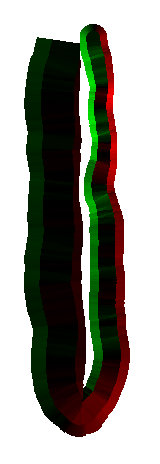
\includegraphics[width=0.25\columnwidth]{\figpath/u_gt}
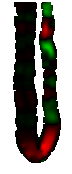
\includegraphics[width=0.25\columnwidth]{\figpath/u_est} &
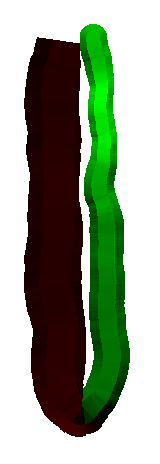
\includegraphics[width=0.25\columnwidth]{\figpath/v_gt}
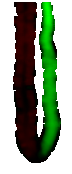
\includegraphics[width=0.25\columnwidth]{\figpath/v_est} \\
(a) & (b)
\end{tabular}}
%
\caption{Qualitative comparison of true flow field with that estimated from optical flow in the (a) horizontal and (b) vertical directions. Hue indicates the direction of flow over the sequence (green is right/down, red is left/up) and intensity is proportional to flow rate (black indicates zero flow).}
\label{fig_flow_results_synth}
\end{figure}
